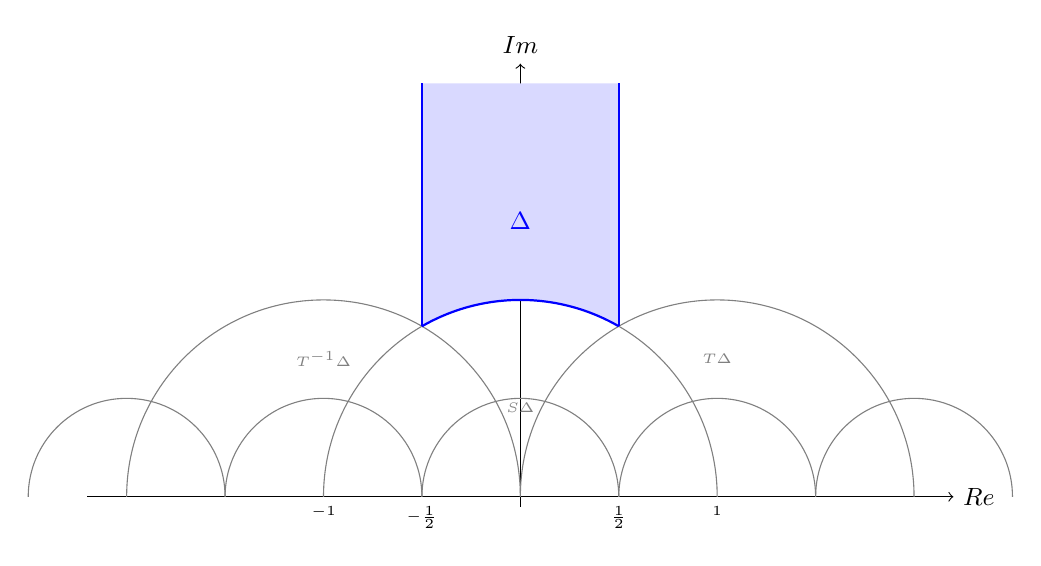
\begin{tikzpicture}[scale=2.5]
    \draw[->] (-2.2, 0) -- (2.2, 0) node[right] {\small\(\operatorname{Re}\)};
    \draw[->] (0, -0.05) -- (0, 2.2) node[above] {\small\(\operatorname{Im}\)};
    \foreach \k in {-2,-1,0,1,2} {
        \draw[gray, thin] ({\k-0.5}, 0) arc (180:0:0.5);
    }
    \foreach \k in {-1,0,1} {
        \draw[gray, thin] ({\k-1}, 0) arc (180:0:1);
    }
    \fill[blue!15] (-0.5, {sqrt(3)/2}) -- (-0.5, 2.1) -- (0.5, 2.1) -- (0.5, {sqrt(3)/2}) arc (60:120:1) -- cycle;
    \draw[blue, thick] (-0.5, {sqrt(3)/2}) -- (-0.5, 2.1);
    \draw[blue, thick] (0.5, {sqrt(3)/2}) -- (0.5, 2.1);
    \draw[blue, thick] (-0.5, {sqrt(3)/2}) arc (120:60:1);
    \node[blue] at (0, 1.4) {\small\(\Delta\)};
    \node[below] at (-0.5, 0) {\tiny\(-\frac{1}{2}\)};
    \node[below] at (0.5, 0) {\tiny\(\frac{1}{2}\)};
    \node[below] at (-1, 0) {\tiny\(-1\)};
    \node[below] at (1, 0) {\tiny\(1\)};
    \node[gray] at (-1, 0.7) {\tiny\(T^{-1}\Delta\)};
    \node[gray] at (1, 0.7) {\tiny\(T\Delta\)};
    \node[gray] at (0, 0.45) {\tiny\(S\Delta\)};
\end{tikzpicture}
